\documentclass{article} % For LaTeX2e
\usepackage{nips15submit_e,times}
\usepackage{hyperref, dsfont,graphicx}
\usepackage{url,subcaption}
%\documentstyle[nips14submit_09,times,art10]{article} % For LaTeX 2.09
\usepackage{bm}

\usepackage{algorithm}

\usepackage[noend]{algpseudocode} 

\title{LART - Laplace Noise and Multiple Additive Regression Trees}


\author{Peter Rindal 
\And
Trung Viet Vu 
\And
Hung Viet Le}

% The \author macro works with any number of authors. There are two commands
% used to separate the names and addresses of multiple authors: \And and \AND.
%
% Using \And between authors leaves it to \LaTeX{} to determine where to break
% the lines. Using \AND forces a linebreak at that point. So, if \LaTeX{}
% puts 3 of 4 authors names on the first line, and the last on the second
% line, try using \AND instead of \And before the third author name.

\newcommand{\fix}{\marginpar{FIX}}
\newcommand{\new}{\marginpar{NEW}}

\nipsfinalcopy % Uncomment for camera-ready version

\begin{document}

 
\maketitle

\begin{abstract}

Boosting is a successful machine learning algorithm for a number of regression and classification tasks. Combined with tree base learner, boosted ensemble algorithms are shown to deliver highly accurate and strong predictive models. In this work, we first study a well-known approach called Multiple Additive Regression Trees (MART). By looking at its weakness, we proposed a different approach named Laplace Additive Regression Trees (LART) to mitigate this by injecting random Laplace noises. We then build on this algorithm by combining it with Dropout meets multiple Additive Regression Tree (DART)\cite{dart} resulting in what we call DLART. In the experiment, we compare the performance of LART, DLART to MART and DART on the dataset that has been used in previous papers. Our results is promising as the proposed LART/DLART methods yield significant gains in accuracy in this particular task.

\end{abstract}

\section{Introduction}

% introduce the problem. See the dart paper for a good intro. We want to frame it as the MART algorithm suffers from later trees not contributing much and that the consecutive trees have too much in common. i.e. the same predicates are often chosen between consecutive tree when the learning rate/shrinkage is small , e.g. 0.05. 

Ensemble modeling is a powerful way to improve the performance of a single learning model.  It can be able to out-perform any single classifier within the ensemble \cite{Dietterich2000}. Many methods for constructing ensembles have been developed. One popular approach is Bagging and Random Forest \cite{Breiman2001}, in which different subsets of the training examples are used to learn independent predictors. Another practical technique is boosting. Boosted algorithms focus on improving the current model by iteratively adjusting the learning algorithm between iterations. In general, this method often results in better reduction in  error and achieving strong predictive models. \\

In 2001, Friedmn \cite{mart} introduced an ensemble of boosted regression trees - MART, which combines boosting with tree base learner. At each iteration a tree is added to fit the gradient using least square. The resulting model forms an ensemble of weak predictive models that gives highly accurate predictions. Later on, Caruana and Niculescu-Mizail \cite{Caruana06anempirical} demonstrated the application of MART to build highly successful models for many learning tasks. Despite its success, this algorithm still suffers from the problem of over-fitting where the learned model does not generalize well to unseen data. This issue is addressed in \cite{VinayakG15} as \textit{over-specialization}: trees added at later iterations tend to have too much in common, and add negligible contribution towards the prediction of all the remaining instances. In real-world settings, the MART algorithm often starts with a single tree that learns the objective of the problem while the additive trees in the ensemble learn the deviation from this objective. In this sense, the ensemble is sensitive to the decision made by the first tree.\\

One commonly used tool to approach the problem of over-specialization in MART is \textit{shrinkage} \cite{mart}. Empirically this regularization technique reduces the impact of each tree by a constant value - \textit{shrinkage factor}, which helps dramatically improve the model's generalization ability. However, while the over-fitting problem can be mitigated by shrinkage, the fundamental issue of over-specialization still remains, i.e. as the size of the ensemble increases, the contribution of the later trees is negligible \cite{VinayakG15}. Motivated by this, we hypothesize that randomizing the process of selecting predicates can provide another effective regularization for MART and propose the LART algorithm.


\subsection{Mart - Random Forest Hybrid}

% maybe one of you can write this. Talk about how our randomization technique allows a smooth transition between a random forest technique and the original MART. This can be tuned and talk about how the use of the laplace random variable effects this randomization. I.e. if one predicate/split is significantly better, then it will still be pick with good probability (assuming a moderate amount of noise.)

In this work, we explore an improvement in MART to address the issue of over-specialization. Specifically, we propose a method called Laplace Additive Regression Trees (LART), which injects randomness into the learning algorithm.
By adding Laplace noises to the calculation of the loss function, a predicate can be sampled in a way such that a greater reduce in the loss function results in it being more likely to be selected. In partiucular, the probability of less desirable predicates being sampled decreases exponentially in proportion to their reduction in loss. Instead of selecting the predicate that simply minimizes the loss function, we select the predicate that minimizes the sum of the loss function and an additive random Laplace variable with appropriate scale. Predicates chosen in this way are more uncorrelated and hence the diversity in the learners increases.\\

One motivation for this approach is a hybrid view between MART and Random Forest. While MART takes the advantage of boosting algorithms in achieving low bias and low variance, it can be sensitive to noise and outliers as mentioned above. On the other hand, Random Forest benefits from the diversity among the learned classifiers and hence it is more robust to noise and outliers. However, it has the major disadvantage of regression trees, that is, their inaccuracy. Our proposed method tries to capture the advantage of these two approaches with appropriate additive Laplace noise. When the Laplace distribution is scaled by too much, the noise will drown out the contribution that the loss function may have. Predicates at each iteration are likely to be chosen randomly. This leads to special case wherein LART is similar to a Random Forest algorithm. Conversely, if the Laplace noise is too small, the loss function will dominate and effectively result in the MART algorithm. Tuning the scale of Laplace noise thus is a major point of investigation for our work.



\subsection{Differential Privacy }

An alternative way to interpret this work is from the perspective of differential privacy. The general setting of differential privacy is that we wish to run an algorithm on some sensitive dataset and reveal the result. Moreover, this result must have privacy guarantees with respect to how much information on \emph{any single record} can be obtained from the result alone. Put another way, places mathematical bounds on the amount of information any example can have on the final model.

While this work is not concerned about privacy, we are concerned with the problem of over fitting which decision trees are particularly susceptible to. Over fitting is a general problem in machine learning where the model learns random errors in the training set as opposed to the underlying distribution. 

In more detail, differential privacy guarantees that for two datasets $X,Y$ where $Y$ has one training example $X$ does not, then the probability that the training algorithm on $X$ and $Y$ will produce the same models should be bounded by
$$
	\forall m \in\mbox{Models} \ : \ \Pr[m = \textsc{Train}(X)] \leq \exp(\epsilon) \Pr[m= \textsc{Train}(Y)]
$$
What this definition says is that the algorithm \textsc{Train} should output the model $m$ with roughly the same probability when the parameter $\epsilon\in (0,\infty]$ is near $0$, i.e. $\exp(\epsilon)\approx 1$. In the case that $\epsilon$ is very large, this definition of differential privacy places no constraint the the output of the algorithm. In the setting of differential privacy, a smaller value for $\epsilon$ is considered more private, e.g. $\epsilon=0.1$. 

Comparing this to the problem of over fitting, we can see many parallels. That is, if $Y = X \cup {y}$ and $y$ is an training example with which significantly deviates from the underlying distribution, then a training algorithm which is differentially privacy will give guarantees about the impact that this outlier can have. This observation is the primary inspiration of this for this work. That is, by observing that over fitting can be framed as allowing a single (or few) example too much impact on the model, differential privacy offers a mathematical framework to limit this influence. 

Later we will discuss how this randomization technique using the Laplace distribution can be used to give the above bound on the impact of any record. However, it should be noted that we do not try to fully satisfy the requirements of differential privacy, instead we apply differentially private techniques in a heuristically manner. Therefore the bound above does not apply in a global sense.

\section{Related Work}    
 
 Gradient boosting is a general technique to build a linear combination of based learners that starts with an initial guessed learner and in each step, adds a single tree to the ensemble learned in the previous step in a linear way to minimize the lost function.  Friedman et al.\cite{mart} adapted the gradient boosting technique to build MART, an ensemble of tree base learners. It has been reported\cite{Caruana06anempirical} to produce highly accurate predictions. But, its main weakness is \textit{over-specialization}:  trees added at later iterations tend to have too much in common, and add negligible contribution towards the prediction of all the remaining instances. We will get back to this problem in more details in Section~\ref{sec:over-spe}. Rashmi and Gilad-Bachrach proposed addressing this problem by using randomization. Specifically, they randomly drop a subset of based learners learned in previous steps out of the current ensemble to train the next ensemble. We propose a different approach of utilizing randomization that incorporate Laplace noise to overcome over-specialization.
 
Regarding injecting randomness into an ensemble of trees, there are roughly two ways~\cite{PV07} in literature: \emph{input randomization} and \emph{feature randomization}. Two extrem representatives of two classes are Bagging~\cite{Breiman96} and Extra-Tree~\cite{GEW06} where Bagging only employs input randomization and Extra-Tree only employs feature randomization.

In input randomization, the original idea is to subsample the training set to obtain $B$ training subsets where each training subset is sampled (with replacement) according to the uniform distribution.  Each training subset is used to train a decision tree and then, trees are aggregated together into a single predictor, thereby reducing the noise effect. Wagging~\cite{BK98} is another variant of input randomization method where each sample is assigned a random weight and all training samples are retained in the training set. Since Bagging can be seen as Wagging where the weights come from discrete Poisson distribution, Webb et al.~\cite{WZ04} proposed assigning weights following continuous Poisson distribution.  

Beside input randomization, there are vast majority of works built upon the idea of feature randomization. Ho~\cite{Ho98} proposed sampling a subset of features, called a subspace, projecting training data on to this subspace and building a decision tree for the projected training data. Thus, each subspace sampling would give a tree and a collection of subspace samples gives a forest. Another idea is to inject randomization in the splitting process while growing the tree. Dietterich~\cite{Dietterich00} proposed an approach that  randomly choose an attribute from a set of potential candidate attributes to split. There could be some flexibility in defining a set of potential candidate attributes and the randomization can also be added to the split value itself~\cite{CZ01,GEW06}. Also, one can use a random linear combination~\cite{Breiman2001} of attributes to determine the split threshold. Our work lies in this (feature randomization) category.
\section{Over Specialization} \label{sec:over-spe}

Over-specialization of MART was identified  by Rashmi and Gilad-Bachrach~\cite{dart} in their work on DART. Essentially, they observed that the added last trees tend to have impact on a small number of instances. As a result, the initial added trees would have a huge contribution to the ensemble. Note that the based tree learners are very simple function of the input and parameters. This causes the negative effect on the performance of the resulting ensemble on unseen data. Though over-specialization can be reduced by \emph{shrinkage}, i.e, multiplying leaf values of each to-be-added tree by a constant value in $(0,1)$, it still persists.  Rashmi and Gilad-Bachrach demonstrated their observation through extensive experiments and argued that over-specialization can be eliminated using randomization.     In Section~\ref{sec:algo}, we introduce a different randomized scheme to overcome this issue.

\section{The Algorithms} \label{sec:algo}

\subsection{Mart}
We begin by describing the Mart\cite{mart} algorithm on which we will build the LART algorithm. The Mart algorithm can be viewed as a (functional) gradient decent algorithm. The model is then constructed iteratively by generating a series of trees, each correcting the previous set. This is done by taking the derivative of the loss function based the current predictions and updates the model by adding another regression tree that is trained to fit the negation of these derivative. 

The input to the algorithm is a labeled dataset $D=\{(x,y)\}$ where $x\in \mathcal{X}$ is a vector in the feature space $\mathcal{X}$ and $y\in \mathcal{Y}$ is the labels in prediction space. In addition to $D$, the algorithm takes as input a loss function $\mathcal{L}_x :  \mathcal{Y} \mapsto \mathds{R} $ which the models the model tries to minimize. In our case, we are performing regression and chose to use the $L2$ loss function and therefore we have $\mathcal{L}_x(\hat{y} ) = (y- \hat{y})^2$, where $y$ is the true label for example $x$.
 
 
The algorithm begins by initializing the current model $M:\mathcal{X}\mapsto \mathcal{Y}$ to some default map. Let $M(x)$ denote the prediction of the model at the feature vector $x$ and $\mathcal{L}'_{(x,y)}(M(x))$ denote the derivative of the loss function at $M(x)$. At each iteration, Mart then creates new dataset datasets $D'=\{(x,-\mathcal{L}'(M(x)))\}$  and learns a new tree model $T$ for $D'$. This tree $T$ is trained to predict the negation of the the derivate of the loss function. The current model is then updated as $M(x):= M(x) + T(x)$, thereby reducing the loss.

In the case of the $L2$ loss function describe above, its derivative is $\mathcal{L}'_{(x,y)}(\hat{y}) = 2(y - \hat{y})$. This will be the loss function of choice in the evaluation section as it is suitable to the regression task in question. However, other loss functions can be defines for different tasks such as classification. In this case, the  the logistic loss function can be used $\mathcal{L}_x (\hat{y}) =( 1 + \exp(\lambda y \hat{y}))^{-1}$ and consecutive models will be trained to fit its derivative.

One problem with this algorithm is that the model can converge too fast, getting stuck in a local optimum. In terms of a tradition gradient decent algorithm, this is akin to have too large of a learning rate. To address this, a common technique known as shrinkage is applied to the models, which reduces the impact any single tree has on the overall ensemble by a constant factor $\lambda\in (0,1]$. In the Experiment section, this will sometimes be referred to as the learning rate or lr for short. Algorithmically,  this shrinkage factor is implemented by updating the model as $M(x):= M(x) + \lambda T(x)$, where $T$ is the three that was just learned.


\subsection{LART}
We now turn our attention to the LART technique discussed in this paper. One problem with the Mart algorithm is that of over specialization as discussed above\cite{dart}. In this case the later trees contribute very little to the  model as trees start to fail to fit the derivative of the loss function. The related work Dart \cite{dart} suggest that randomizing how these trees are constructed can provide some benefit in that later trees continue to improve the model. While they put forth a technique based on dropout, our technique is based on methods from differential privacy.


First let turn our attention to how an individual tree $T$ is trained. It is assumed that there exists a set of $m$ predicates the $i$th one $P_i:\mathcal{X} \mapsto \{0,1\}$ map a feature vector to a single bit.  Initially, all records in the training set $D'$ are mapped to the root of the tree. The tree is then recursively constructed by selecting a leaf node $L$. For each predicate $P_i$, the records $(x,y)\in L$ are mapped to $L$'s newly created ``candidate" children $L_{i,0},L_{i,1}$, where $(x,y)$ is mapped to $L_{i,P_i(x)}$. For each of these candidate nodes $L_{i,b}$, the label $\hat{y}_{i,b}$ that minimizes the loss function $\mathcal{L}$ when applied to $(x,y)\in L_{i,b}$ is computed. The pair of leaf nodes $L_{i,0}, L_{i,1}$ which has the greatest reduction in the loss function compared to $L$ is then selected and $L_{i,0}, L_{i,1}$ are added to the tree as leaf nodes. This process of selecting and splitting leaf nodes continues until some stop condition it reached, e.g. the best $k$ leaves have been split.

The LART algorithm randomizes this process of selecting predicates in the following way. Instead of strictly selecting the leaf node pair $L_{i,0}, L_{i,1}$ with the greatest reduction in the loss function, we noisily select the best predicate. In particularly, for each predicate we sample a random variable $\eta\gets \mathcal{D}$ and computed the split's ``effective" reduction in the loss function as $\ell + \eta$, where $\ell$ was the original reduction. The predicate that has the greatest effective reduction in the loss function is then chosen. Although we don't show the derivation, it is equivalent choose $i$ as   
$$
	\arg \max_i \frac{(\sum_{(x,y)\in L_{i,0}} y)^2}{|L_{i,0}|} + \frac{(\sum_{(x,y)\in L_{i,1}} y)^2}{|L_{i,1}|} + \eta
$$ 


%
%\begin{algorithm}
%	
%	\caption{The LART algorithm}\label{alg:LART}
%	
%	\begin{algorithmic}[1]
%		
%		\State Let M be the total number of trees to be added to the ensemble each.
%		
%		\State $F_0(\bm x) = \arg \min_\gamma \sum_{i=1}^N {L(y_i,\gamma) } $ 
%		
%		\For{$m$ = 1 to $M$}
%		
%		\State $\hat{y_i} = - [\frac{\partial L(y_i, F(\bm x_i))}{\partial F(\bm x_i)}] |_{F(\bm x) = F_{m-1}(\bm x)}$, $i=1\ldots N$
%		
%		\State $\bm a_m = \arg \min_{\bm a}  \sum_{i=1}^N {[\hat{y_i} -  h(\bm x_i;\bm a)]^2}$
%		
%		\State $\rho_m = \arg \min_{\rho}  \sum_{i=1}^N {\Big( L(y_i, F_{m-1}(\bm x_i) + \rho h(\bm x_i ; \bm a_m)) + \eta_i^m \Big)}$ \Comment{$\eta_i^m \leftarrow \mathcal{D}$}
%		
%		\State $F_m(\bm x) = F_{m-1}(\bm x) + \lambda \rho_m h(\bm x ; \bm a_m)$ \Comment{$\lambda$ is the shrinkage factor}
%		
%		\EndFor
%		
%		\State \textbf{Output } 
%		
%	\end{algorithmic}
%	
%\end{algorithm}

The choice of the distribution $\mathcal{D}$ can therefore have a significant impact on the performance of the model. In the case that $\ell \ll \eta$ with high probability,  the LART algorithm is identical to a random forest with an appropriate choice of when to stop the algorithm. However, in the case that $\ell \gg \eta$, the LART algorithm is identical to the original Mart algorithm. As such, this modification to the training process allow us to explore the the space of algorithms between Mart and random forest.

In our experimental evaluation we chose to instantiate this distribution $\mathcal{D}$ as the Laplace distribution centered at zero and scaled by $\frac{\mu}{\epsilon}$, where $\mu$ is the mean value of the labels at the leaf and $\epsilon$ is a parameter that allows the amount of noise to be tuned. This choice was made so that in expectation the amount of noise added to the loss function is roughly proportional to the effect of adding/removing $\frac{1}{\epsilon}$ random records to/from the node in question. 



As discussed in the introduction, another way to interpret this modification is that it is a relaxed instance of the Report Noisy Max\cite{Dwork} algorithm from differential privacy. As such, this approximately\footnote{To fully obtain differential privacy, the laplace distribution must be scaled by $\frac{ \Delta\mathcal{L}}{\epsilon}$, where $\Delta\mathcal{L}$ is the maximum change in the loss function that adding any record can have. However, when tuning the LART algorithm, we found that mean behaved better.} give us that for any pairs of datasets $X,Y$ where $Y$ has one additional record as compared to $X$, then the probability that the next split will result in the same predicate $P_i$ on both datasets can be bounded as
$$
	\Pr[i = \textsc{Split}(X)] \leq \exp(\epsilon)\Pr[i =\textsc{Split}(Y)]
$$
As such, this process of adding Laplace noise with an appropriate value for $\epsilon$ can be seen as a way to regularize the impact that and single record can have on the learning process, e.g. outliers. In addition, this randomization technique can also force the trees to become more diversified which can help prevent over-specialization.

\subsection{DART}

To be self contained, we now describe DART\cite{dart} which is a different way to randomize the MART algorithm by performing the randomization on the ADA Boosting portion as opposed to randomizing single trees. The general technique is called dropout and achieves a similar effect to shrinkage/gradient decent learning rate. Both the MART and LART algorithm compute the loss function derivative  which consecutive trees learn as $D'=\{(x,-\mathcal{L}'(M(x)))\}$, where $M(x) =\lambda \sum_{i=1}^n T_i(x)$ and $n$ is the number of tree that have been learned. However, DART ``mutes'' a random subset of the trees at each iteration, resulting in the next training set being $D'=\{(x,-\mathcal{L}'(M'(x)))\}$ where $M'(x) = \sum_{i\in I} \rho_i {T_i(x)} $ and $I\subset \{1,...,n\}$, where $\rho_i$ is a scaling factor for the $i$th tree. The  $(n+1)$th tree that is computed using $D'$ then ``relearn" the tree that were muted at this iteration. To prevent the model from over shooting the function, the new tree and muted trees are normalized, reducing the values $\rho_{n+1}$ and $\rho_i$ for $i\in \{1,...,n\}-I$. We refer the reader to \cite{dart} for a more detailed explanation of the algorithm.

\subsection{DLART}

Due to LART randomizing the individual trees and DART randomizing the boosting operation, it is natural to combine these approaches. In that we add Laplace noise to each of predicate loss function scores and perform the dropout technique of DART. We implement this algorithm and report its performance next.

\section{Evaluation}

We evaluate the our LART technique by comparing it to the Mart, and Dart\cite{dart} algorithms. We additionally compare to a hybrid between LART and DART that we call DLART. We implemented each of their algorithms within our own framework. 

For the dataset, we choose to use the CT slice dataset from \cite{graf20112d} which can be found at \cite{uci_ctSlice}. This dataset contains 53500 histograms created from CT scans of 74 individuals. The task is to locate the position that the scan was taken. Each image is represented as 386 features. We used 10-fold cross validation to compare our algorithm. As with the prior work that we compare to \cite{dart}, we ensure that the splits are chosen such that each individual is completely in the test or training datasets. While Dart\cite{dart} also compare to this dataset, the numbers we get are slightly different than what they report. We suspect that this difference is from how we pre-process the dataset, reducing the number of predicates for each feature to only 4, testing if the feater is greater than $v\in\{0,0.25,0.5,0.74\}$.


\begin{figure}	\centering
	
\begin{subfigure}{.49\textwidth}
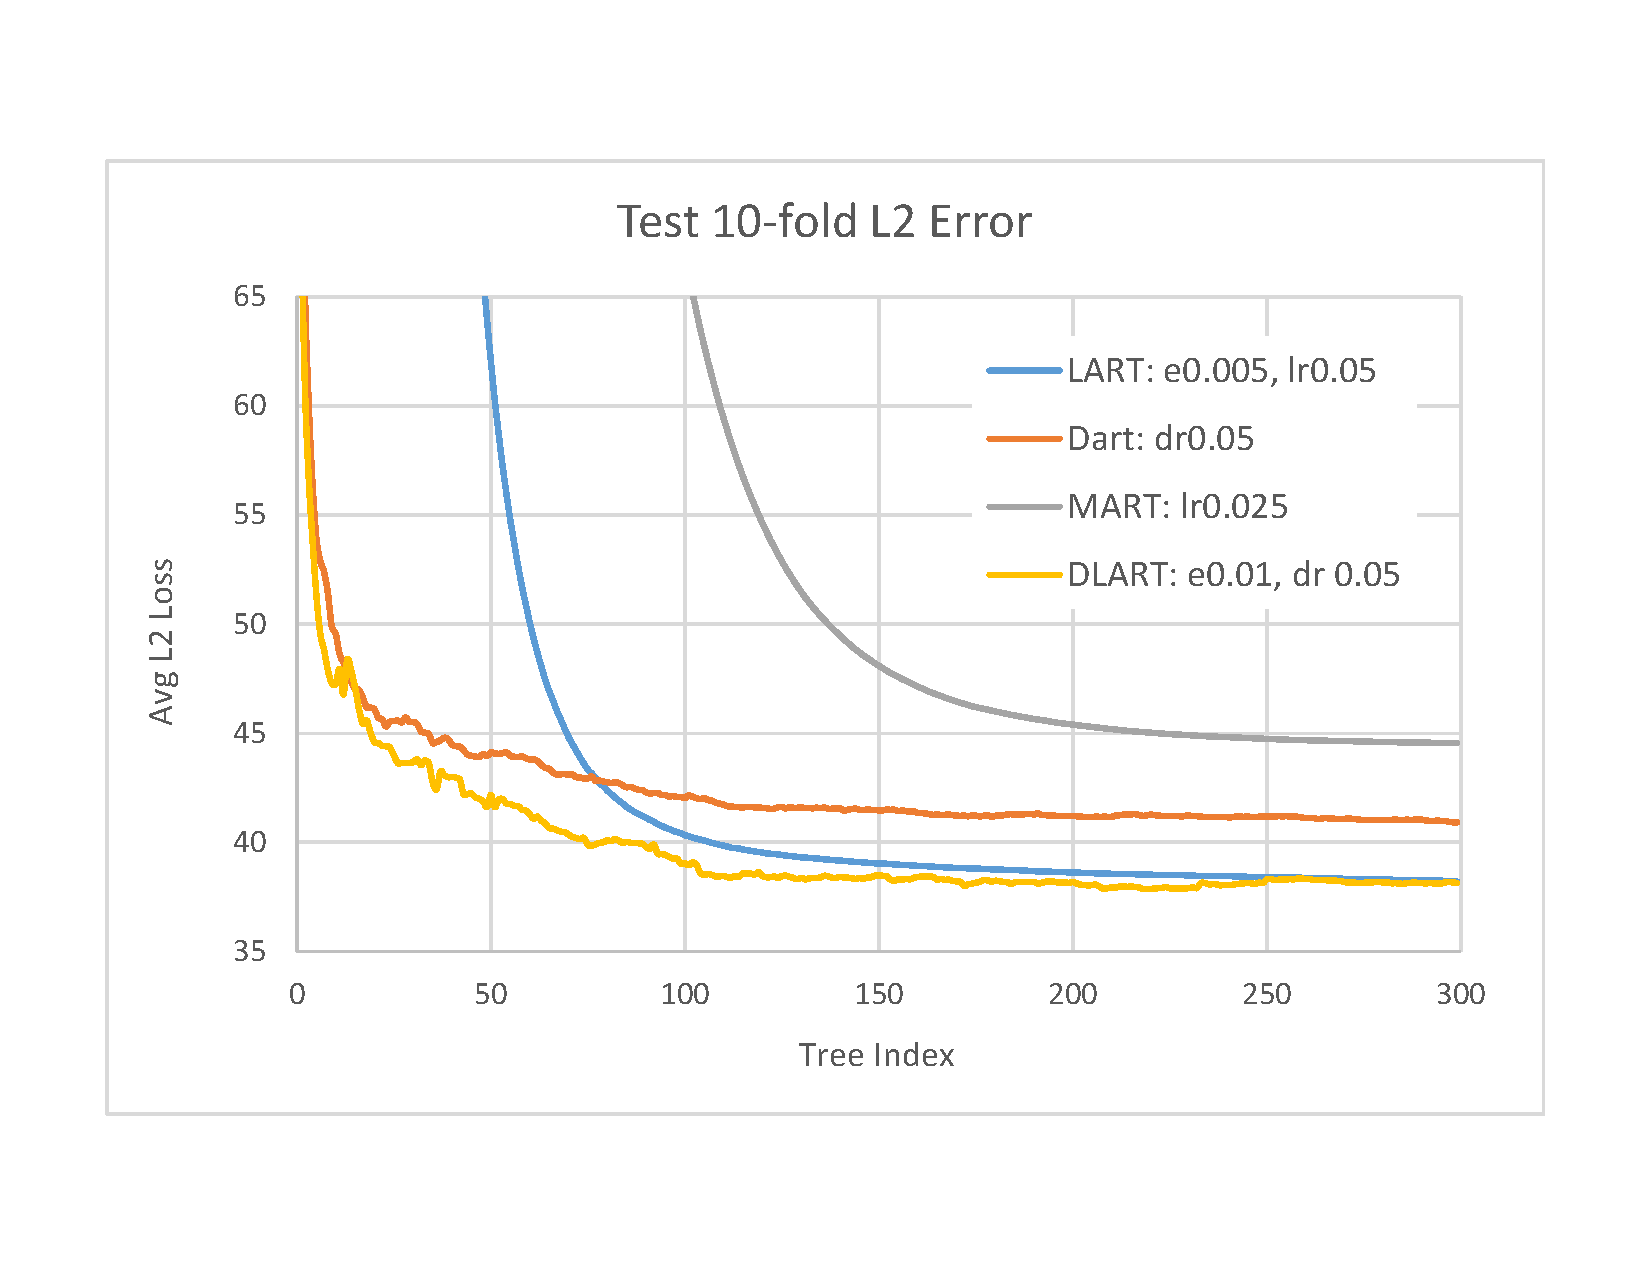
\includegraphics[trim={1.5cm 2cm 1.5cm 2cm},clip, scale = 0.28]{laplaceTree.pdf}
\caption{Average L2 error across all 10 folds versus\\ the number of trees  with a target of 300 trees. \label{fig:compareA}}
\end{subfigure}
\begin{subfigure}{.49\textwidth}
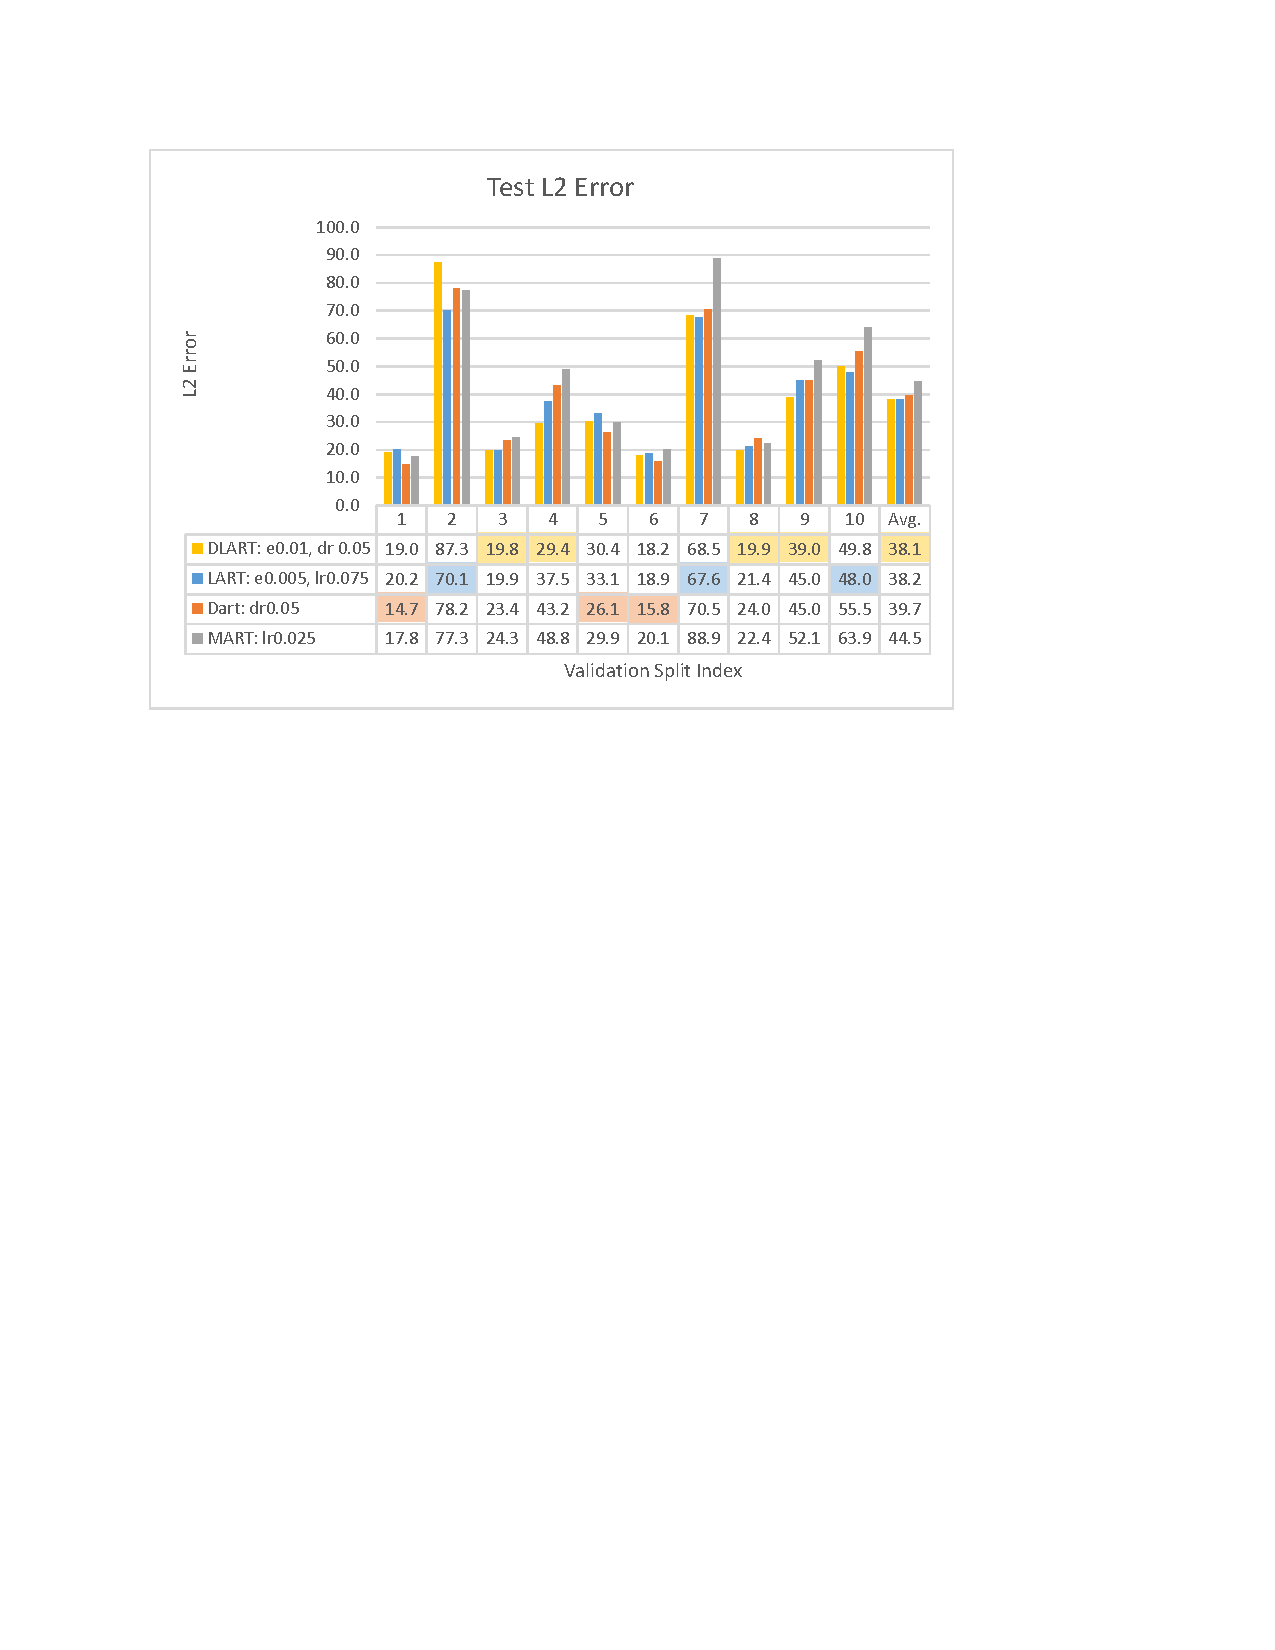
\includegraphics[trim={2cm 15.5cm 5cm 2.1cm},clip, scale = 0.478]{barTable.pdf}
\caption{L2 error on each fold and average for optimal parameters with 300 trees.\label{fig:compareB}}
\end{subfigure}
\caption{Experimental results of comparing MART, LART, DART, DLART. All results shown are the result of a 10-fold cross validation parameter sweep with optimal parameters shown here.  \label{fig:compare}}


\end{figure}

Figure \ref{fig:compare} show the performance of the LART and DLART technique as compared to Mart, Dart. Parameters under consideration were shrinkage $\lambda\in\{0.15, 0.1,0.075, 0.05, 0.025 \}$, Laplace noise scaler $\epsilon\in \{ 1, 0.1,0.05, 0.01, 0.005, 0.001 ,0.0005,0.0001, 0.00005\}$, and drop rate  $dr\in \{0.1, 0.05, 0.01, 0.05, 0.0001\}$. Due to time constraints the large amount of time required to do a parameter sweep, we fixed  the number of trees to be 300 and the number of leaves on each tree to be at most 1000. To make the leaf node restriction efficient, we only split the nodes that result in the best reduction in the (noise) loss function with respect to all splits between the leaves.

As can be seen in Figure \ref{fig:compareA}, LART significantly out performs both DART and MART by a reduction in L2 error of  6.3 and 1.5 respectively. While it can be seen in Figure \ref{fig:compareB} that DART out performed LART on some of the folds, on average the LART randomization technique improved the overall accuracy. The DLART algorithm  combining both the LART and DART techniques achieves the best overall performance with a final L2 error of 38.1, a small reduction in over the LART algorithm alone. 

However, adding the dropout technique has other advantages over LART alone. Most notable is that the DLART algorithm converges to a small L2 error much sooner than LART. This is due to how the the shrinkage effect the learning. In the examples above, a shrinkage of $\lambda=0.05$ for LART and $\lambda=0.025$ for MART were used. This means, after the first tree is constructed, only a $\lambda$ factor of the tree's prediction effects the error. As such, it take many trees to drive the error down. Moreover, if $\lambda$ is increased, the local optimum that the model converges to becomes worse making this effect somewhat inherent to the shrinkage approach. 

On the other hand, the dropout technique does not use shrinkage. Instead, the first tree is taken at its full prediction. On consequential iteration, when a tree is muted and another tree relearns it, the contribution that the muted trees (and new tree) are reduced. In effect, the shrinkage is performed more on-demand, allowing only a few tree giving good accuracy without sacrificing the accuracy obtained when adding more tree. 

\begin{figure}	\centering
	

	
\end{figure}
\section{Conclusions}
In this project, we first review the approach of using Multiple Additive Regression Trees (MART) to regression and classification tasks. The weakness of MART is trees added at later iterations have significantly diminishing contributions. By injecting some randomness to generating ensembles classifiers, we propose a different approach, called LART, to provide efficient regularization for MART. Our experiment shows that LART out-performs MART and the previous best algorithm DART. Moreover, when combining LART with DART we get a highly accurate ensemble that converges quickly. This strengthen our hypothesis that LART is more robust to over-specialization.\\

This study also suggests some point of investigation. One direction is tuning the scale parameter along with other traditional parameters in MART and examining their interaction. Additionally, we might evaluate the performance of LART on more complicated datasets and other machine learning tasks, as in data mining.



\nocite{*}
\bibliographystyle{plain}
\bibliography{ref}


\end{document}
